% Chapter Template

\chapter{A WEB-BASED PROTOTYPE FOR REMOTE CAR DIAGNOSTICS} % Main chapter title

\label{Chapter4} % Change X to a consecutive number; for referencing this chapter elsewhere, use \ref{ChapterX}

\lhead{Chapter 4. \emph{A WEB-BASED PROTOTYPE FOR REMOTE CAR DIAGNOSTICS}} % Change X to a consecutive number; this is for the header on each page - perhaps a shortened title

%----------------------------------------------------------------------------------------
%	SECTION 1
%----------------------------------------------------------------------------------------
\section{About the application}
This application is a prototype for remote car diagnostics and control, basically is a web app built with a responsive front-end because the target devices are smartphones.
The car is simulated by a car toy made with raspberry pi (Figure \ref{fig:Raspberry}) and a car chassis development kit (Figure \ref{fig:car_chassis}). 

\subsubsection{Dashboard}
Into the dashboard (Figure \ref{fig:dashboard}) we can see main levels and temperatures from the car, all dates are storage into a NoSQL database, so you can see some history of the oil level for example, the dates are dummy data for now just some random numbers.
\newpage
\begin{figure}[h!]
  \centering
    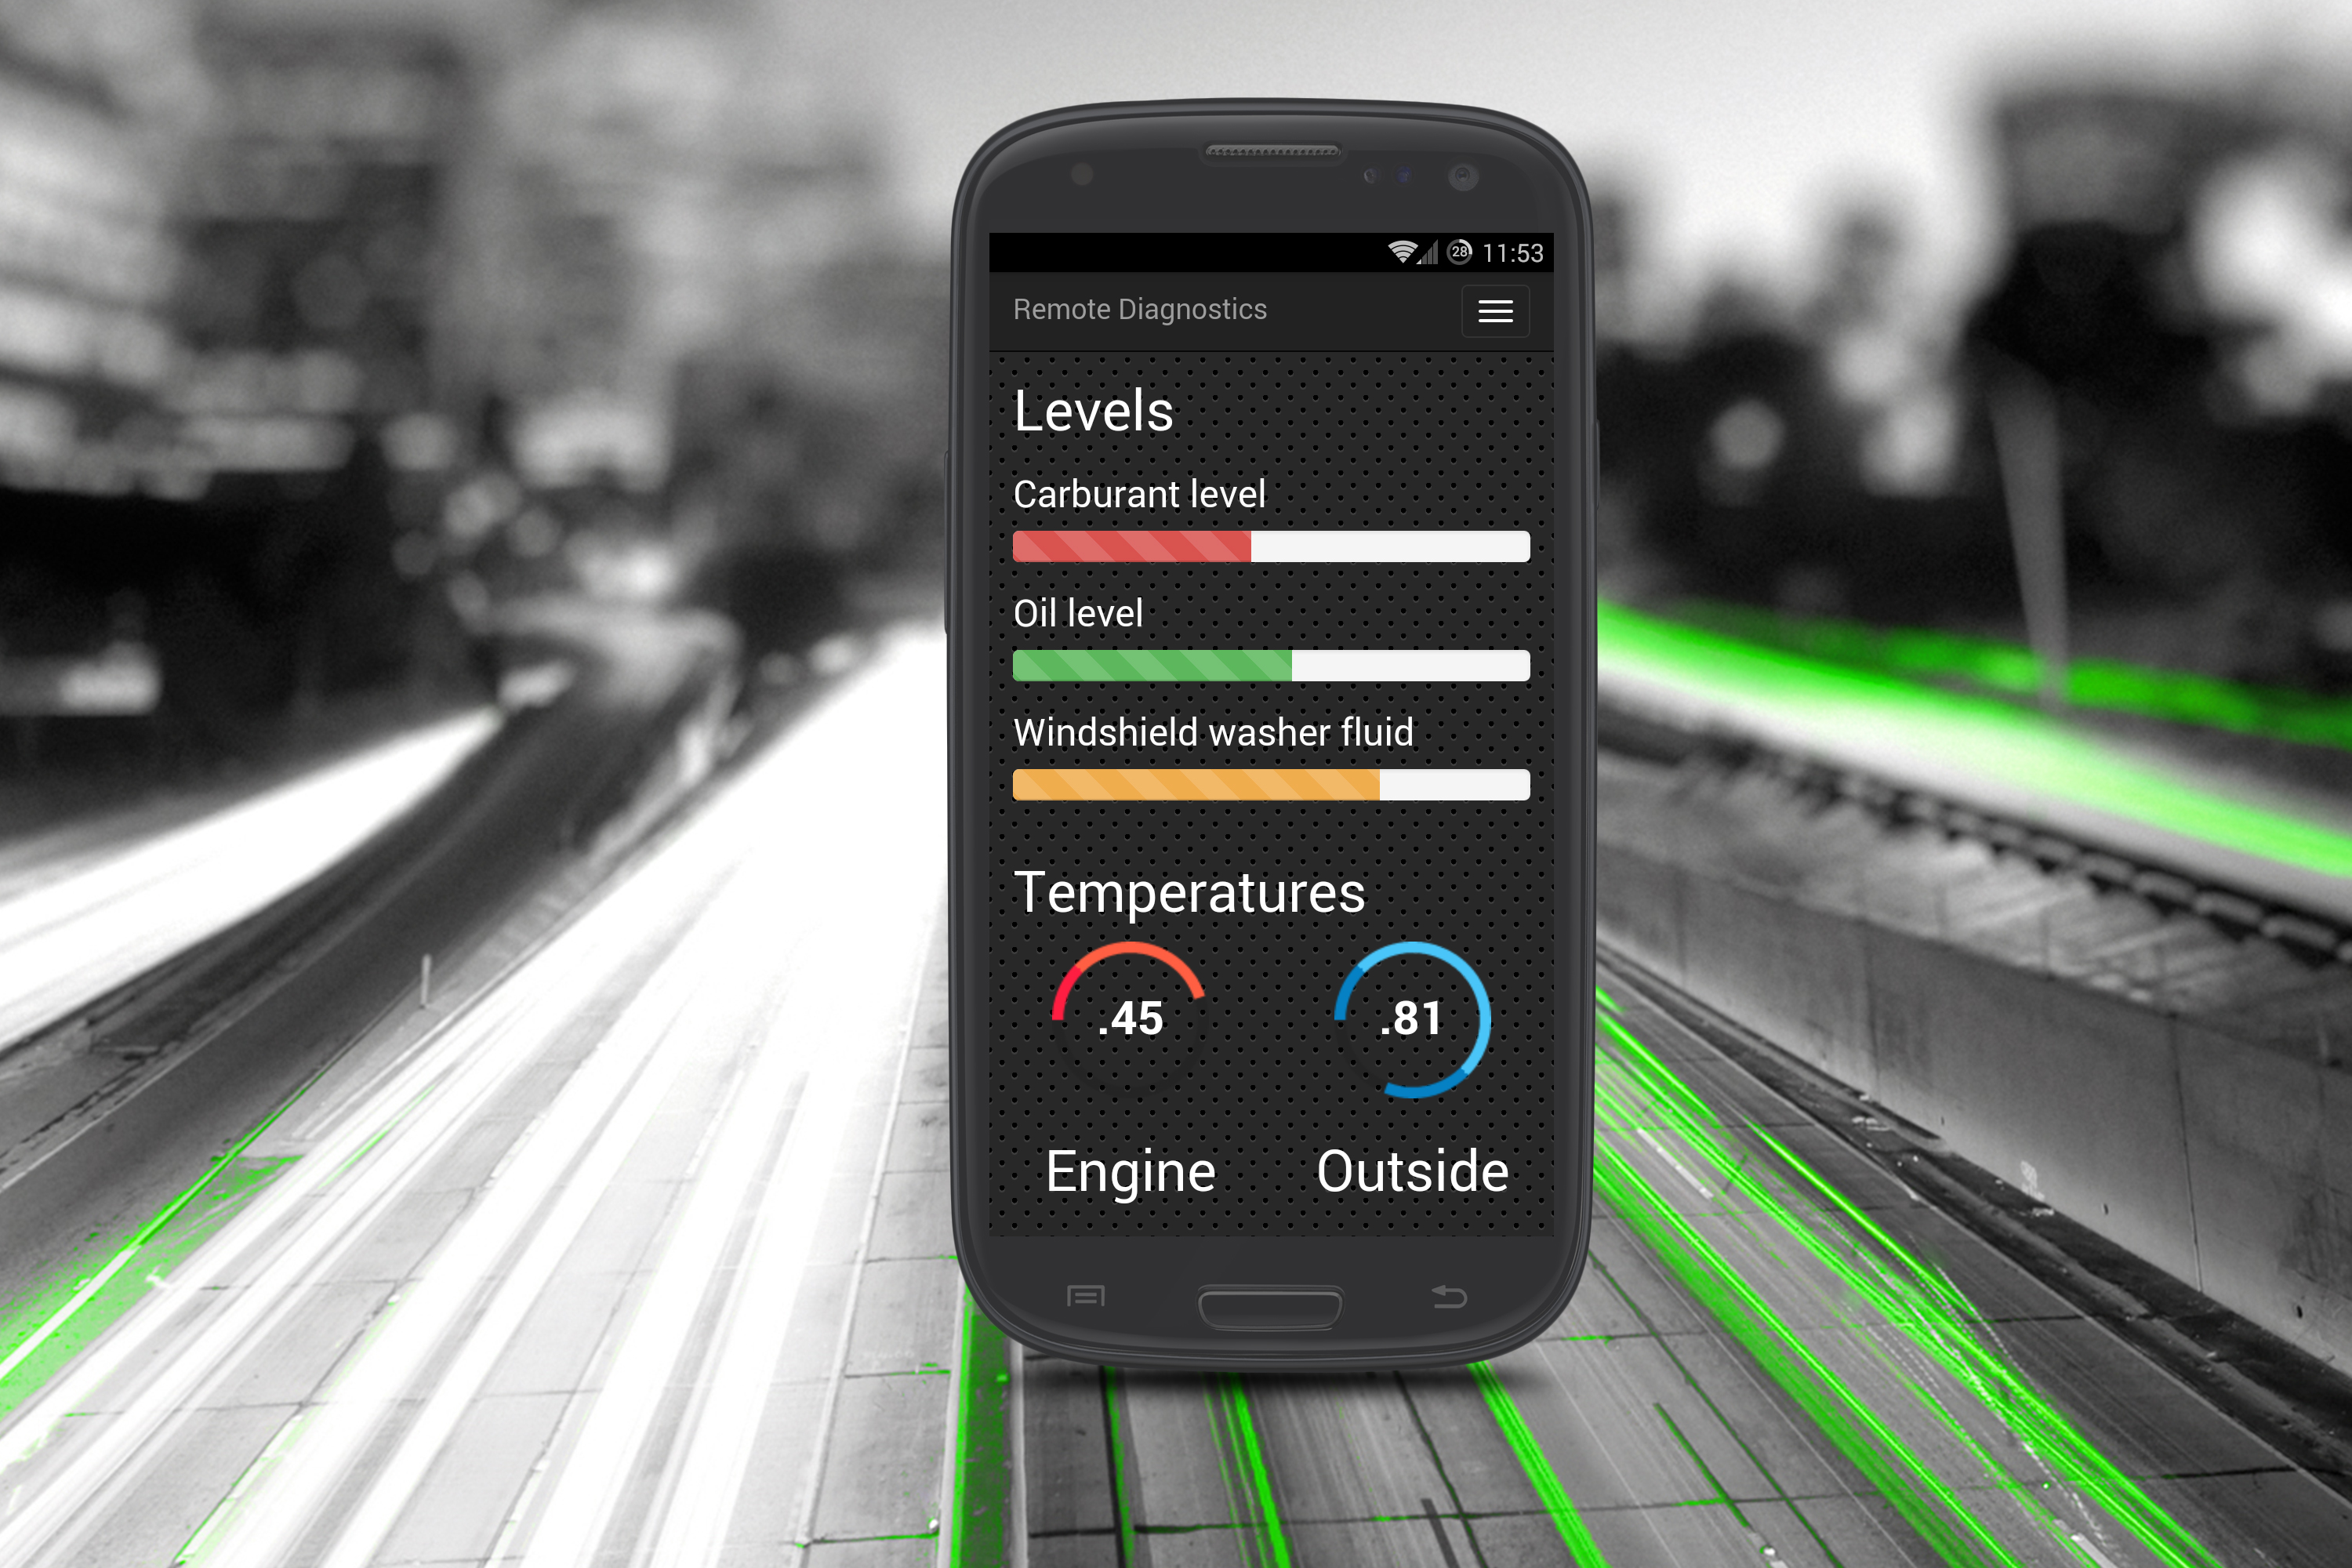
\includegraphics[width=1\textwidth]{./Pictures/dashboard.jpg}
  \rule{1\textwidth}{1pt}
 \caption{Dashboard}
  \label{fig:dashboard}
\end{figure}
%-----------------------------------
%	SUBSECTION 1
%-----------------------------------
\subsection{Controllers}
For the remote control of the car i made three kind of controllers:
\begin{itemize}
  \item Keyboard Controller (Figure \ref{fig:keyboard_controller})
  \item Gyroscope Controller (Figure \ref{fig:gyroscope_controller}) 
  \item Speech Controller (Figure \ref{fig:speech_controller})
\end{itemize}
\subsubsection{Keyboard Controller}
The keyboard controller (Figure \ref{fig:keyboard_controller}) is pretty simple, just press the direction where you want to direct the car.

\subsubsection{Gyroscope Controller}
For controling the car with the gyroscope controller(Figure \ref{fig:gyroscope_controller}) grab the phone with the display facing upwards and incline front,back,left and right to stop just keep the phone horizontally. 


\subsubsection{Speech Controller}
With this controller just ``talk''  with the phone some simple commands like ``left'',``right'',``up'',``down'' and ``stop''.(Figure \ref{fig:speech_controller})

\begin{figure}[h!]
  \centering
    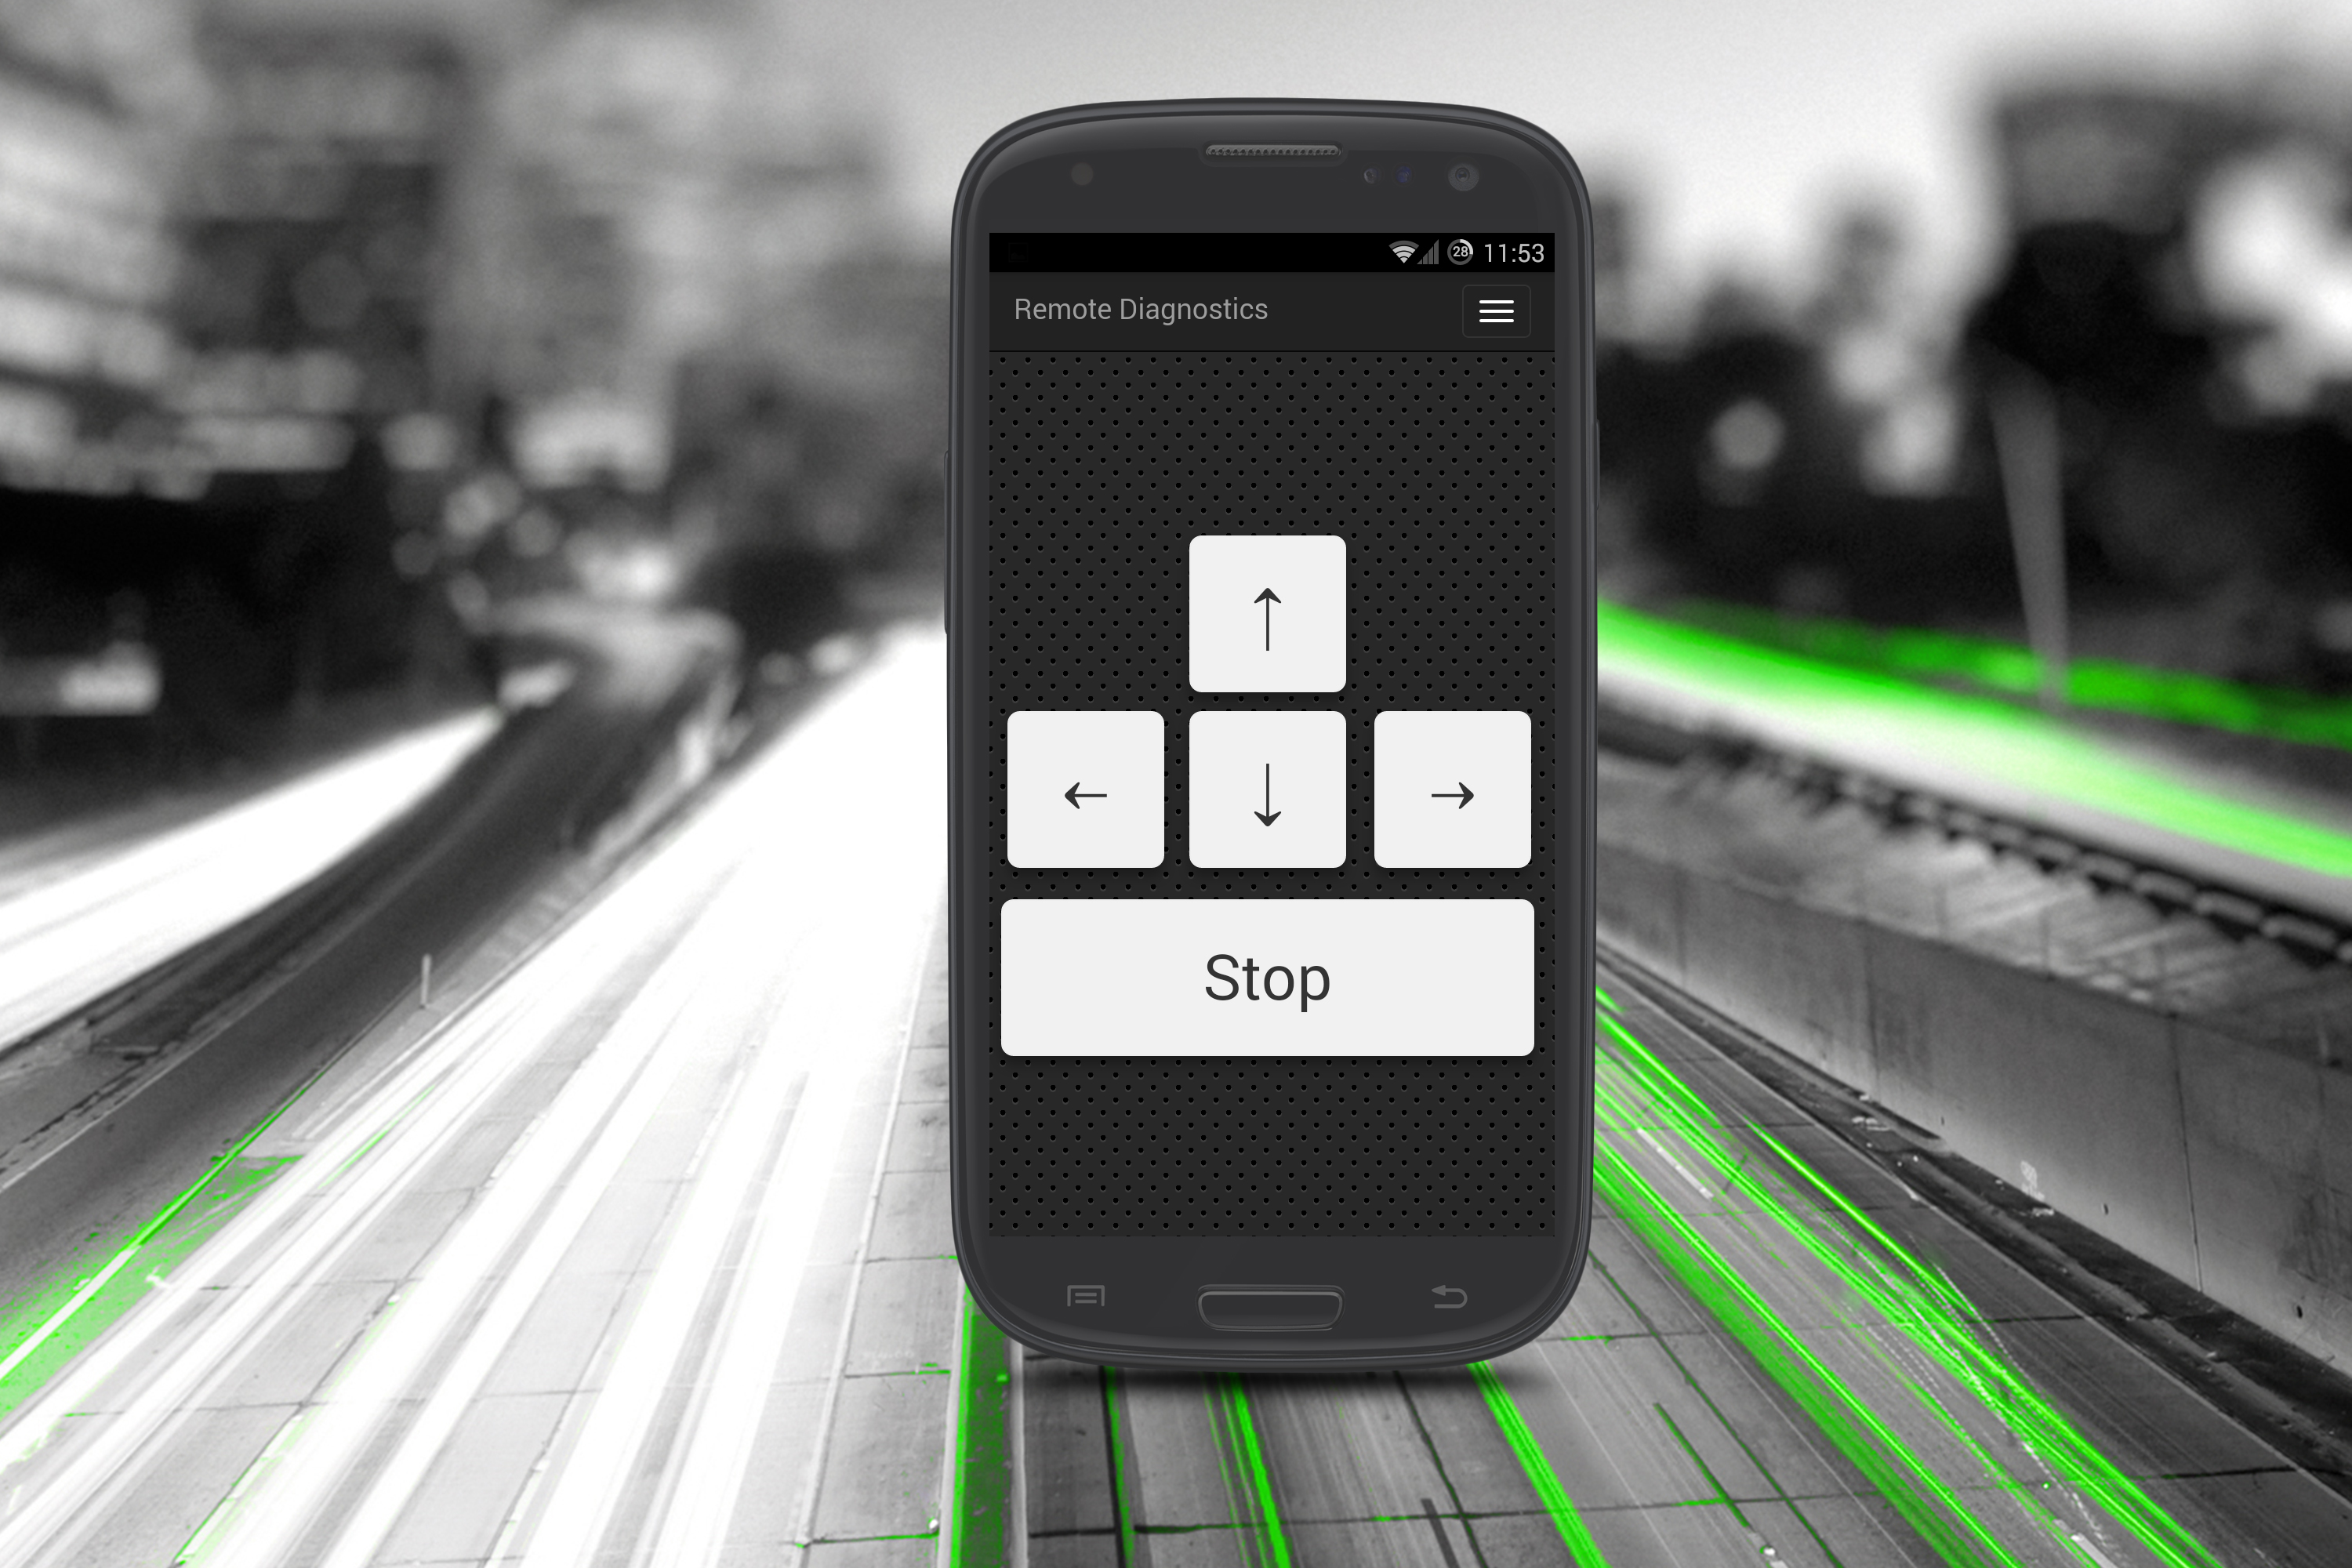
\includegraphics[width=1\textwidth]{./Pictures/keyboard_controller.jpg}
  \rule{1\textwidth}{1pt}
 \caption{Keyboard Controller}
 \label{fig:keyboard_controller}
\end{figure}
\begin{figure}[h!]
  \centering
    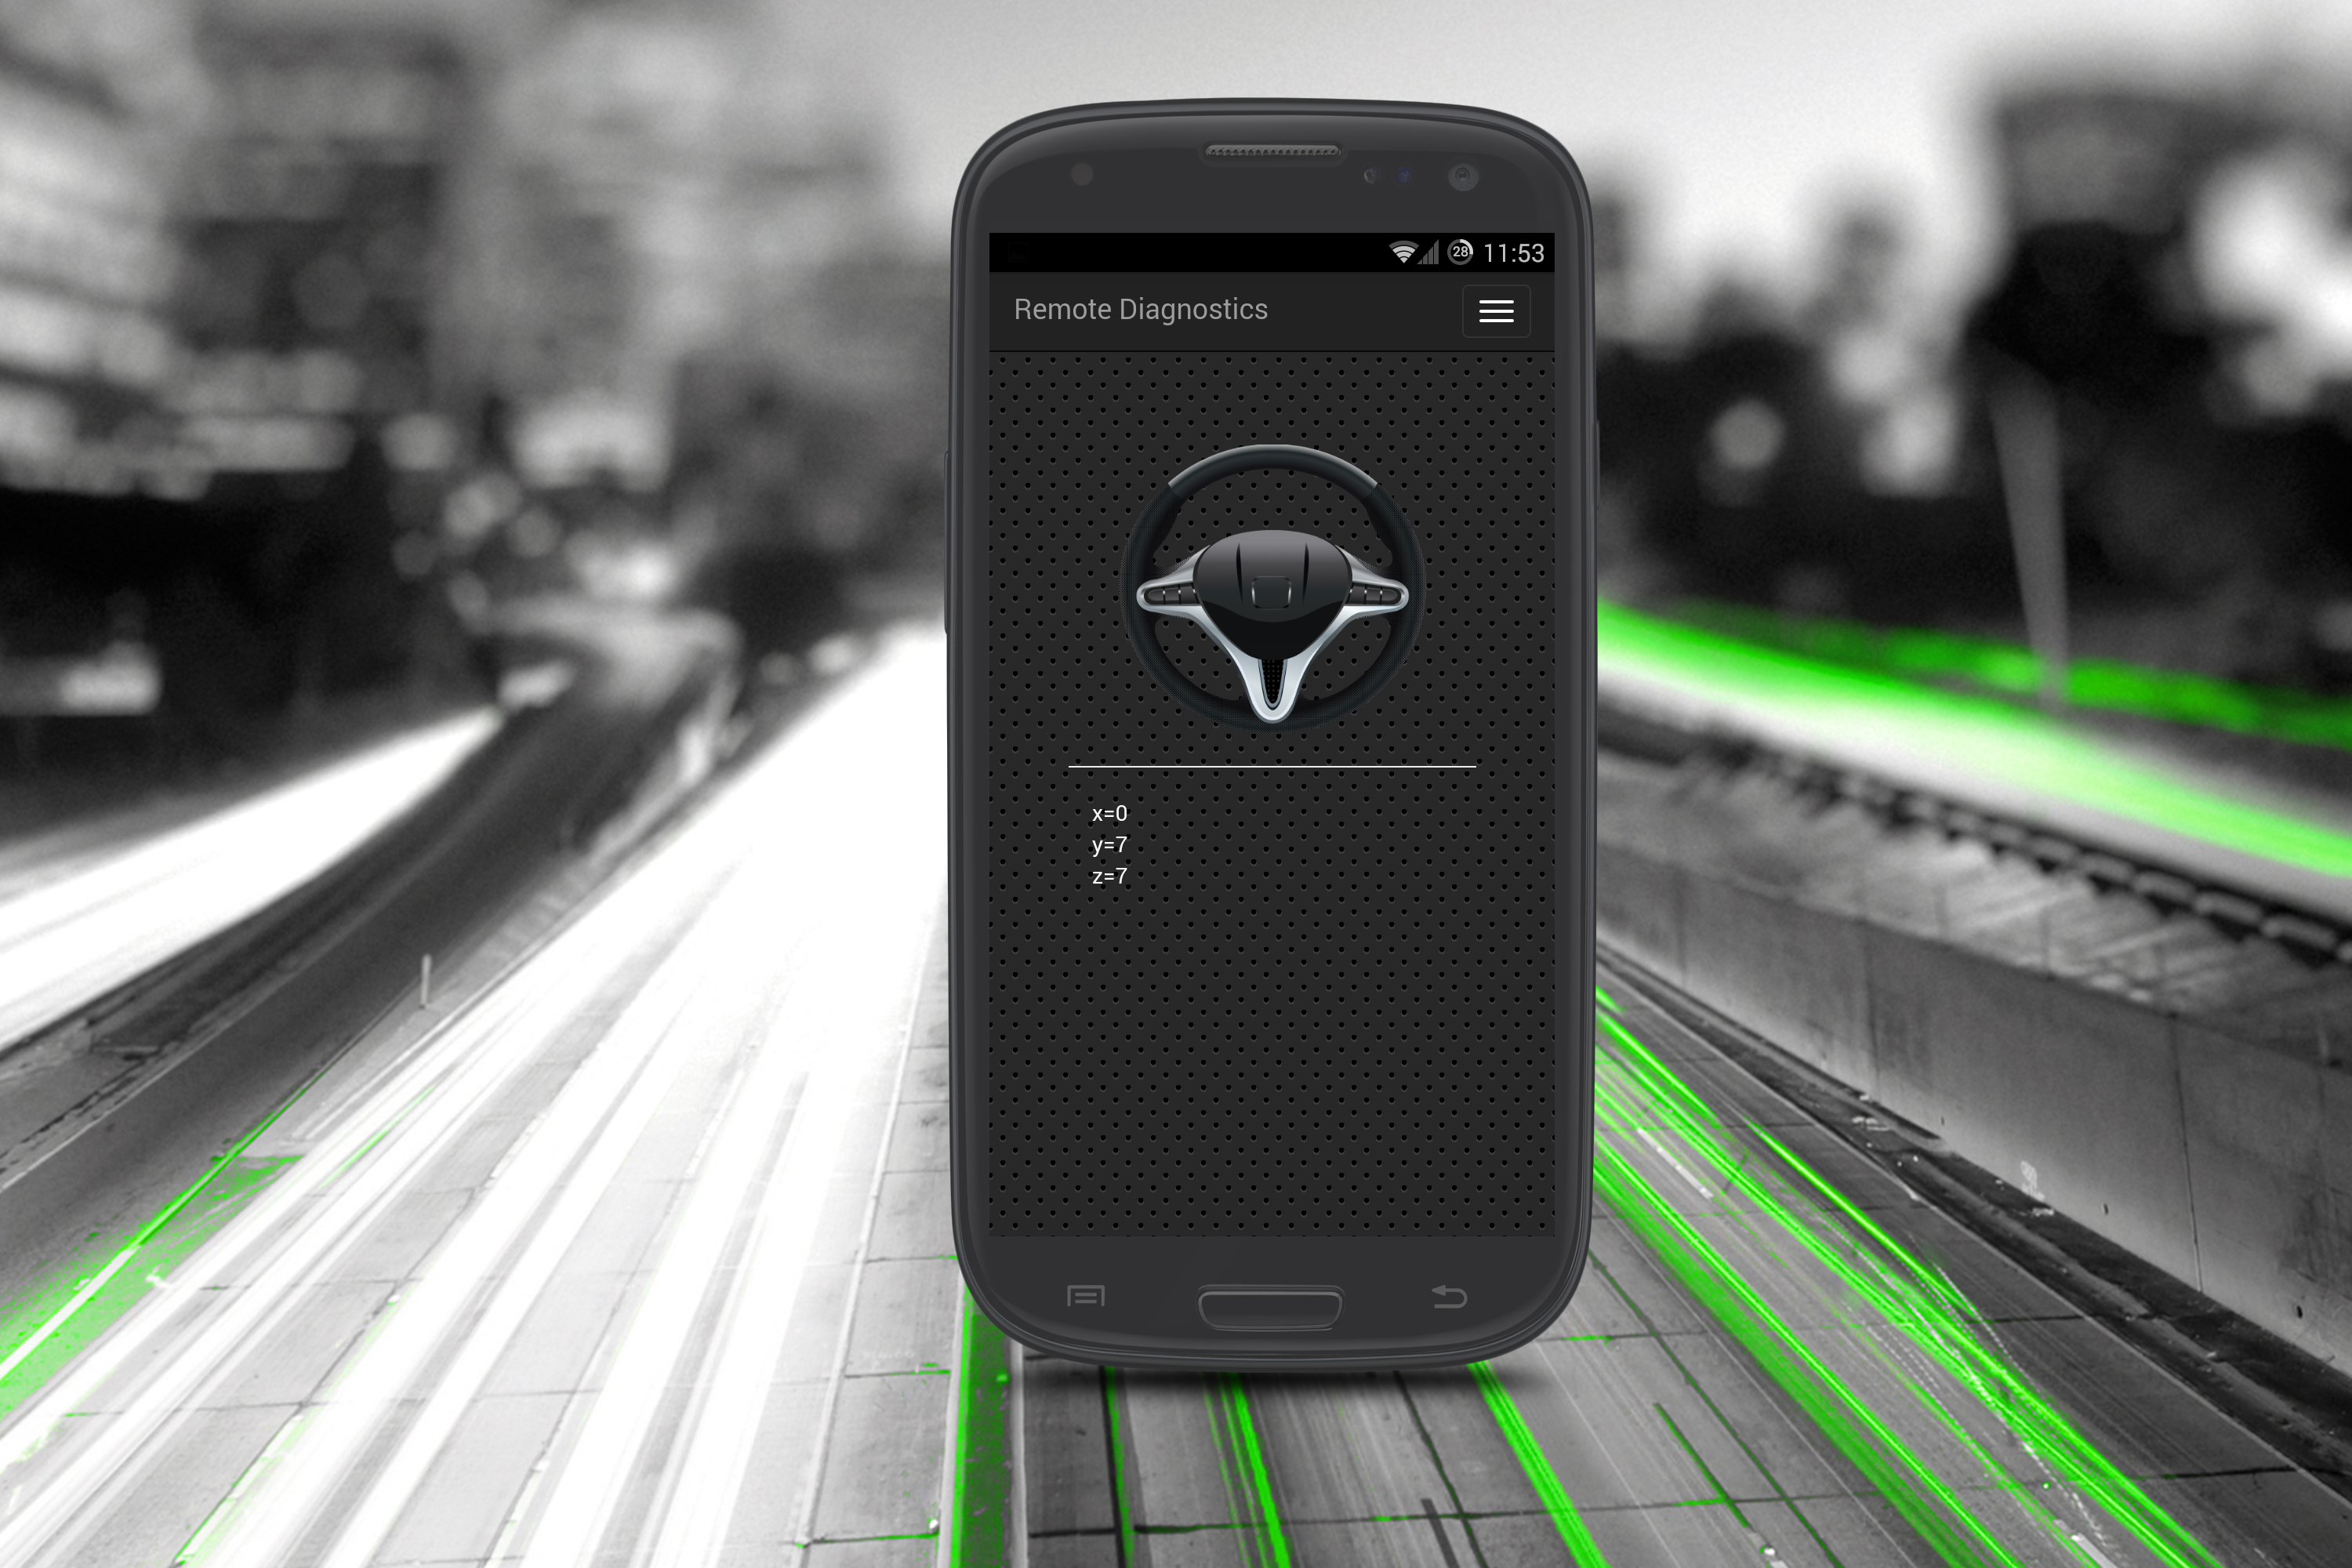
\includegraphics[width=1\textwidth]{./Pictures/gyroscope_controller.jpg}
  \rule{1\textwidth}{1pt}
 \caption{Gyroscope Controller}
  \label{fig:gyroscope_controller}
\end{figure}
\begin{figure}[h!]
  \centering
    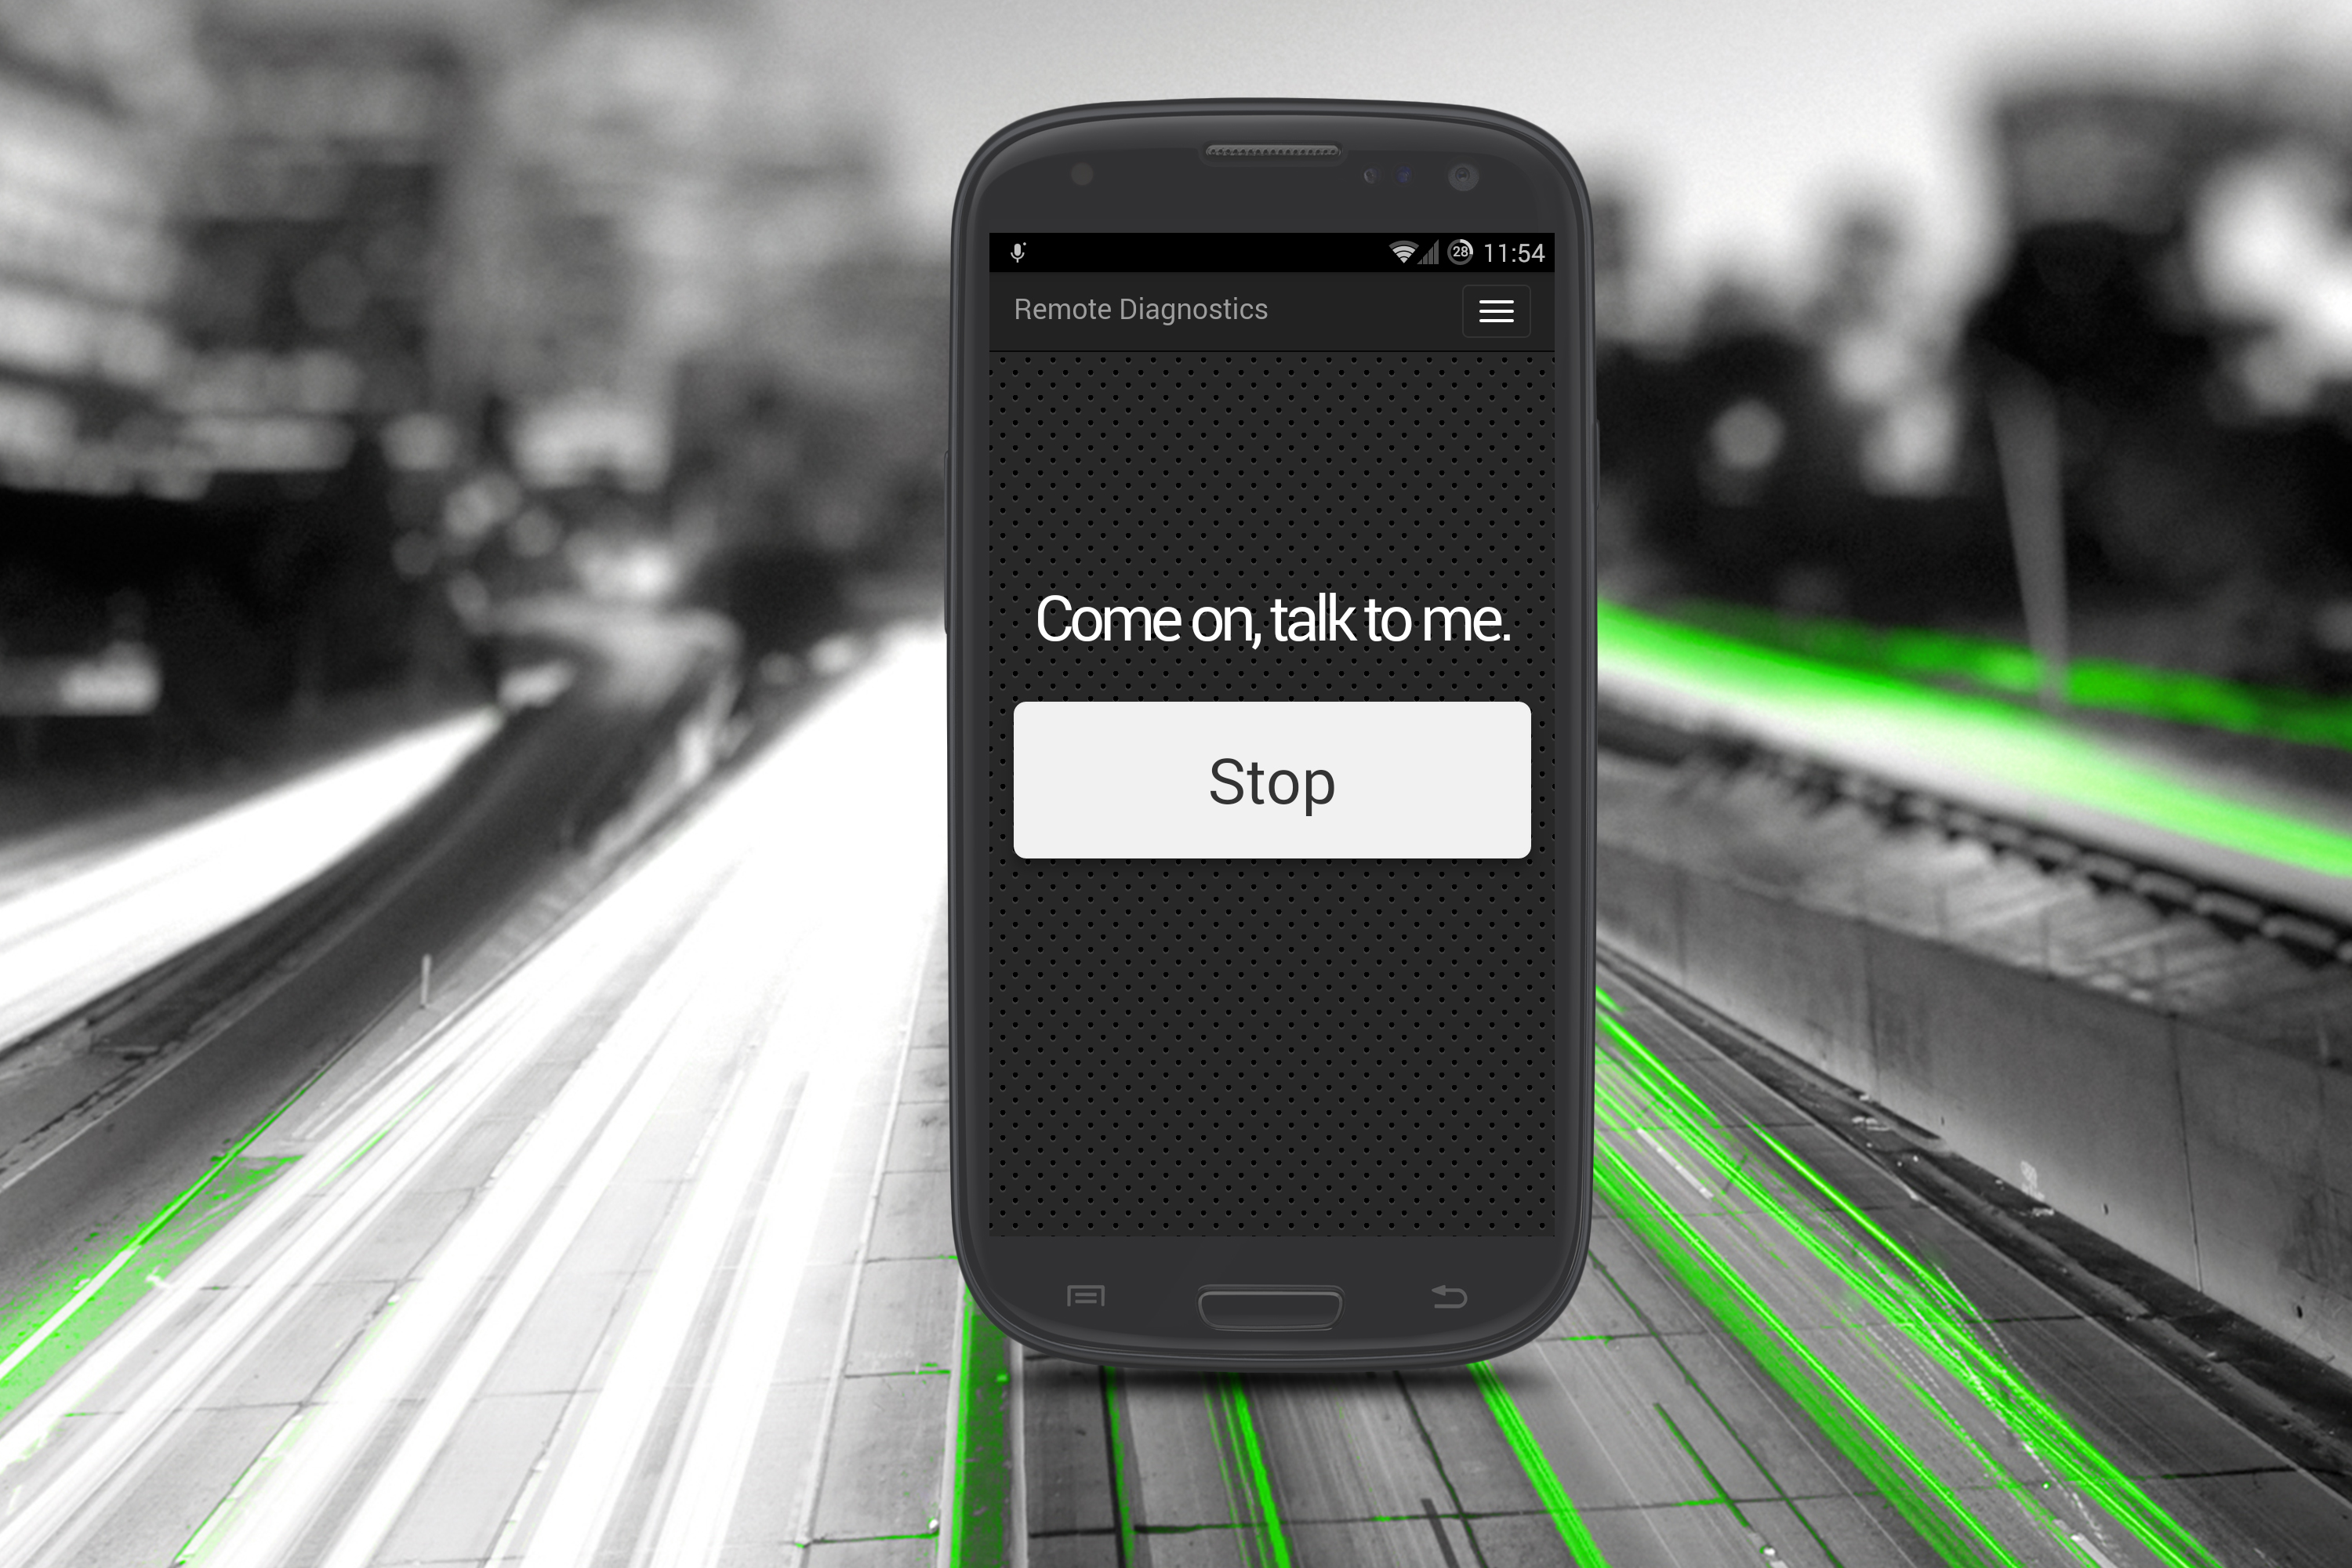
\includegraphics[width=1\textwidth]{./Pictures/speech_controller.jpg}
  \rule{1\textwidth}{1pt}
 \caption{Speech Controller}
  \label{fig:speech_controller}
\end{figure}

\newpage
\clearpage
%-----------------------------------
%	SUBSECTION 2
%-----------------------------------
\section{How?}
\paragraph*{Why node.js?}
I choose node js because i like JavaScript and this is the most popular language at this moment for web development, and with node js you can write javascript for the back-end of the app not just for front-end in conclusion: JavaScript everywhere!



To install node.js just download node from \url{ https://nodejs.org/}(Figure \ref{fig:nodejsorg}).

\begin{figure}[h!]
  \centering
    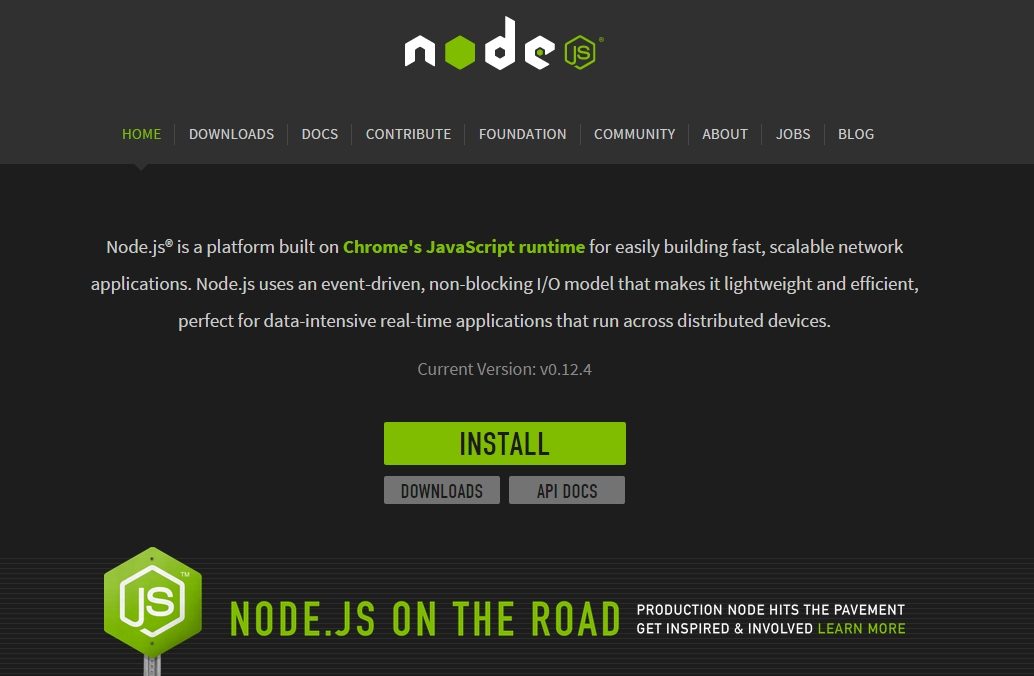
\includegraphics[width=1\textwidth]{./Pictures/nodejsorg.jpg}
  \rule{1\textwidth}{1pt}
 \caption{https://nodejs.org/}
  \label{fig:nodejsorg}
\end{figure}

After open the terminal and check the node version taping: 
\begin{lstlisting}
$ npm -v
\end{lstlisting}
The actual version is 0.12.4.
\paragraph*{Hello World with Node.js}
\hfill \break
Here, the obligatory Hello World example uses Node.js. Write the following line in a
file called \textit{helloworld.js} and save it:
\begin{lstlisting}
console.log("Hello World");
\end{lstlisting}
And now to run it, execute the following command:
\begin{lstlisting}
node helloworld.js
\end{lstlisting}
\paragraph*{AN EXAMPLE: WEBSERVER}
\hfill \break
This simple web server written in Node responds with "Hello World" for every request.
Write the following line in a
file called \textit{exemple.js} and save it:
\begin{lstlisting}[language=JavaScript]
var http = require('http');
http.createServer(function (req, res) {
  res.writeHead(200, {'Content-Type': 'text/plain'});
  res.end('Hello World\n');
}).listen(1337, '127.0.0.1');
console.log('Server running at http://127.0.0.1:1337/');
\end{lstlisting}
And now to run it, execute the following command:
\begin{lstlisting}
node exemple.js
\end{lstlisting}
And open the browser at \url{http://127.0.0.1:1337/}

\paragraph*{Install Express.js}
\hfill \break
First, create a directory to hold your application, if you haven’t already done so, and make that your working directory.
\begin{lstlisting}
$ mkdir myapp
$ cd myapp
\end{lstlisting}
Create a \textit{package.json} file in the directory of interest, if it does not exist already, with the npm init command.
\begin{lstlisting}
$ npm init
\end{lstlisting}
Install Express in the app directory and save it in the dependencies list:
\begin{lstlisting}
$ npm install express --save
\end{lstlisting}
\paragraph*{Express application generator}
\hfill \break
Use the application generator tool, express, to quickly create a application skeleton.

Install it with the following command.
\begin{lstlisting}
$ npm install express-generator -g
$ express myapp
   create : myapp
   create : myapp/package.json
   create : myapp/app.js
   create : myapp/public
   create : myapp/public/javascripts
   create : myapp/public/images
   create : myapp/routes
   create : myapp/routes/index.js
   create : myapp/routes/users.js
   create : myapp/public/stylesheets
   create : myapp/public/stylesheets/style.css
   create : myapp/views
   create : myapp/views/index.jade
   create : myapp/views/layout.jade
   create : myapp/views/error.jade
   create : myapp/bin
   create : myapp/bin/www
\end{lstlisting}
Then install dependencies:
\begin{lstlisting}
$ cd myapp 
$ npm install
\end{lstlisting}
And now start the app with:
\begin{lstlisting}
$ npm start
\end{lstlisting}
Then load \url{http://localhost:3000/} in your browser to access the app.

Add all dependecies used in this project, open packege.json and paste at dependencies object.

\begin{lstlisting}[language=JavaScript]
  "dependencies": {
    "body-parser": "~1.12.0",
    "bootstrap": "~3.3.4",
    "chartist": "^0.8.3",
    "connect-flash": "0.1.x",
    "cookie-parser": "~1.3.4",
    "debug": "~2.1.1",
    "express": "~4.12.2",
    "jade": "~1.9.2",
    "jquery": "~2.1.4",
    "less-middleware": "1.0.x",
    "morgan": "~1.5.1",
    "nosql": "^3.0.2",
    "onoff": "^1.0.2",
    "passport": ">= 0.0.0",
    "passport-local": ">= 0.0.0",
    "python-shell": "^0.1.0",
    "screenfull": "^2.0.0",
    "serve-favicon": "~2.2.0",
    "socket.io": "~1.3.5",
    "watchjs": "0.0.0"
  },
\end{lstlisting}
Install dependecies with this command
\begin{lstlisting}
$ npm install
\end{lstlisting}

\section{My code contribution}
\subsection{Controling the car with Keyboard Controller}
\subsubsection{gpio controller.js}

\begin{lstlisting}[language=JavaScript]
var Gpio = require('onoff').Gpio,
    wra = new Gpio(17, 'out');
    wrb = new Gpio(27, 'out');
    wla = new Gpio(22, 'out');
    wlb = new Gpio(23, 'out');
function up() {
    console.log("up");
    wra.write(1);
    wrb.write(0);   
    wla.write(0);
    wlb.write(1);
}
function down() {
    console.log("down");
    wra.write(0);
    wrb.write(1);   
    wla.write(1);
    wlb.write(0);
}
function left() {
    console.log("left");
    wra.write(1);
    wrb.write(0);   
    wla.write(1);
    wlb.write(0);
}
function right() {
    console.log("right");
    wra.write(0);
    wrb.write(1);   
    wla.write(0);
    wlb.write(1);
}
function stop() {
    console.log("stop");
    wra.write(0);
    wrb.write(0);   
    wla.write(0);
    wlb.write(0);
}
exports.user_left = function() {
    stop();
};
exports.moving = function(move) {
    switch (move["move"].val) {
        case "up":
            if (move["move"].data == "true") {
                up();
            } else {
                stop();
            };
            break;
        case "down":
            if (move["move"].data == "true") {
                down();
            } else {
                stop();
            };
            break;
        case "left":
            if (move["move"].data == "true") {
                left();
            } else {
                stop();
            };
            break;
        case "right":
            if (move["move"].data == "true") {
                right();
            } else {
                stop();
            };
            break;
        case "stop":
            stop();
            break;
    }
};
\end{lstlisting}
\subsubsection{back-end keyboard controller.js}
\begin{lstlisting}[language=JavaScript]
var express = require('express');
var router = express.Router();
// var app = require('../app');
var io = require('socket.io').listen(4000);
var gpio_controller = require('./gpio_controller.js');
var ultrasonicsensor = require('./ultrasonicsensor.js');
router.get('/', function(req, res, next) {
    res.render('keyboard_controller', {
        title: 'Keyboard Controller'
    });
});
io.sockets.on('connection', function(socket) {
    socket.on('moving', function(data) {
        gpio_controller.moving(data);
    });
    socket.on('disconnect', function() {
        gpio_controller.user_left();
    });
});
module.exports = router;
\end{lstlisting}
\subsubsection{front-end keyboard controller.js}
\begin{lstlisting}[language=JavaScript]
var socket = io.connect(':4000');
var move = {
    "data": '',
    "val": ''
};

function send(move) {
    socket.emit('moving', {
        move
    });
    return false;
};
$(document).ready(function() {
    $('#up').bind('touchstart', function() {
        $(this).css({
            'background-color': '#1AFF00'
        });
        move.data = "true";
        move.val = "up";
        send(move);
    });
    $('#up').bind('touchend', function() {
        $(this).css({
            'background-color': '#F1F1F1'
        });
        move.data = "false";
        move.val = "up";
        send(move);
    });
    $('#down').bind('touchstart', function() {
        $(this).css({
            'background-color': '#1AFF00'
        });
        move.data = "true";
        move.val = "down";
        send(move);
    });
    $('#down').bind('touchend', function() {
        $(this).css({
            'background-color': '#F1F1F1'
        });
        move.data = "false";
        move.val = "down";
        send(move);
    });
    $('#left').bind('touchstart', function() {
        $(this).css({
            'background-color': '#1AFF00'
        });
        move.data = "true";
        move.val = "left";
        send(move);
    });
    $('#left').bind('touchend', function() {
        $(this).css({
            'background-color': '#F1F1F1'
        });
        move.data = "false";
        move.val = "left";
        send(move);
    });
    $('#right').bind('touchstart', function() {
        $(this).css({
            'background-color': '#1AFF00'
        });
        move.data = "true";
        move.val = "right";
        send(move);
    });
    $('#right').bind('touchend', function() {
        $(this).css({
            'background-color': '#F1F1F1'
        });
        move.data = "false";
        move.val = "right";
        send(move);
    });
    $('#stop').bind('touchstart', function() {
        $(this).css({
            'background-color': 'red'
        });
        move.data = "true";
        move.val = "stop";
        send(move);
    });
    $('#stop').bind('touchend', function() {
        $(this).css({
            'background-color': '#F1F1F1'
        });
    });t
});
\end{lstlisting}
\subsubsection{view keyboard controller.jade}
\begin{lstlisting}[language=JavaScript]
extends layout
block head
	link(rel='stylesheet', href='/stylesheets/keyboard_controller.css')
block content
	.container#keyboard
		ul
			li(unselectable='on')#up &uarr;
				| &#x9;
			li(unselectable='on')#left &larr;
				| &#x9;
			li(unselectable='on')#down &darr;
				| &#x9;
			li(unselectable='on')#right &rarr;
			li(unselectable='on')#stop Stop
block footer
	script(src='./javascripts/keyboard_controller.js')
\end{lstlisting}.

\subsubsection{How they work together}
You need to have the phone and the pi in the same network.

\begin{figure}[h!]
  \centering
    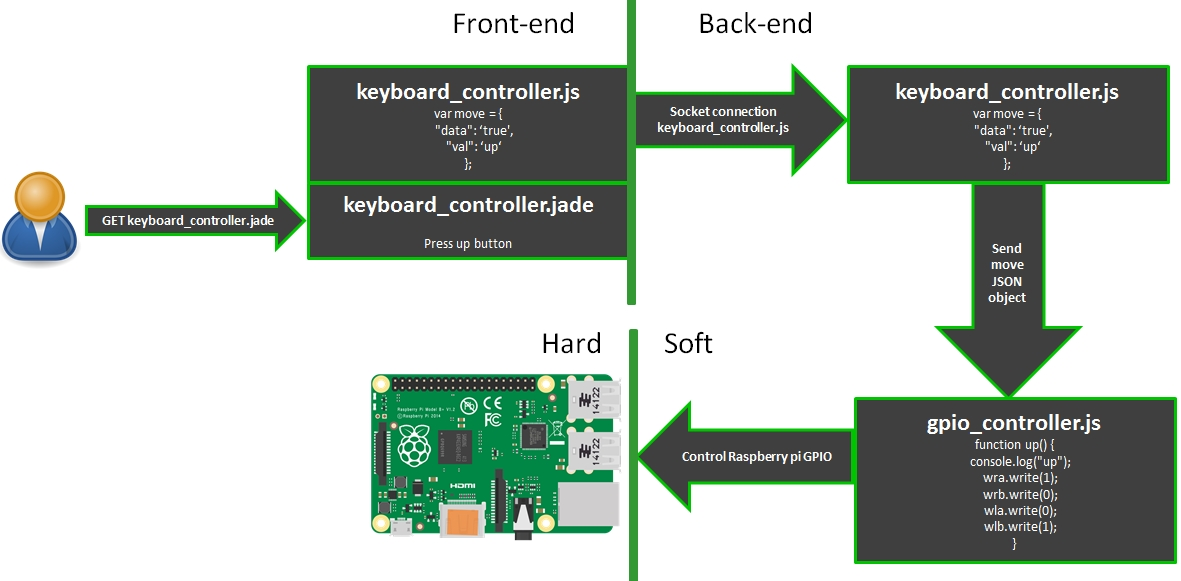
\includegraphics[width=1\textwidth]{./Pictures/controller_workflow.jpg}
  \rule{1\textwidth}{1pt}
 \caption{Keyboard Controller Workflow}
 \label{fig:keyboard_controller}
\end{figure}